\section{Grundlagen}
\label{sec:basics}

In dieser Sektion werden die Technologien, welche die Grundlage für das Monitoring Tool darstellen, kurz erläutert. Für jede dieser Technologien wird die Motivation und die grundsätzliche Funktionalität erklärt.

\subsection{Power-over-Ethernet (PoE)}
\label{sec:poe}
Mit Power-over-Ethernet (PoE) ist es möglich, dass man Geräte über die oft schon vorhandenen Netzwerkkabel mit Strom versorgen kann. Die Idee dahinter, warum man sich überhaupt darüber Gedanken gemacht hat, war dass es eine Menge Geräte gibt die eigentlich eine geringe Stromversorgung brauchen, diesen Strom jedoch durch einen Anschluss an der Stromversorgung des Gebäudes tilgen. Was bedeutet: Überall wo man einfache Netzwerkgeräte braucht (Print-Server, Voice-over-IP Geräte, etc.) braucht man immer sowohl Netzwerk- als auch Stromkabel.

Mittels PoE können die zusätzlichen Stromkabel eingespart werden, sofern das Gerät eine Ladung über das Netzwerk-Interface erlaubt. Dies eignet sich sehr gut für einige eher einfache Geräte wie Webcams, Handhelds, etc.

Für PoE wurden bisher zwei IEEE Standards verabschiedet. Tabelle \ref{tab:compareIeee} zeigt einen kurzen Vergleich zwischen den beiden Standards.

\begin{table}[h]
 \centering
 \begin{tabular}{|c|c|c|c|}
   \hline
   \textbf{IEEE Nummer} & \textbf{Bezeichnung} & \textbf{Leistung / Port} & \textbf{nutzbare Leistung} \\
   \hline
   IEEE 802.3af & PoE & 15,4 Watt & ca. 12,9 Watt \\
   \hline
   IEEE 802.3at & PoE+ & 60 Watt & ca. 51 Watt \\
   \hline
 \end{tabular}
 \caption{Vergleich IEEE Standards \cite{poe2}}
 \label{tab:compareIeee}
\end{table}

Die nutzbare Leistung unterscheidet sich deshalb von der Leistung / Port, weil hier auch der Verlust der bei den RJ-45 Steckern passiert und auch den Verlust über eine Strecke von 100 Metern eingerechnet wurde.

\subsubsection{IEEE 802.3af}
Dieser Standard funktioniert nur mit 10Base-T und 100Base-TX Verbindungen. Die Idee hinter diesem Standard ist, dass man die freien Aderpaare (bei diesen beiden Verbindungen werden nur 2 der 4 Paare verwendet) für die Stromübertragung verwendet. Dieses Verfahren wird \emph{Spare-Pairs-Verfahren} genannt. Abbildung \ref{fig:spare-pairs} zeigt den Aufbau dieses Verfahrens.

\begin{figure}[h]
    \centering
    \leavevmode
    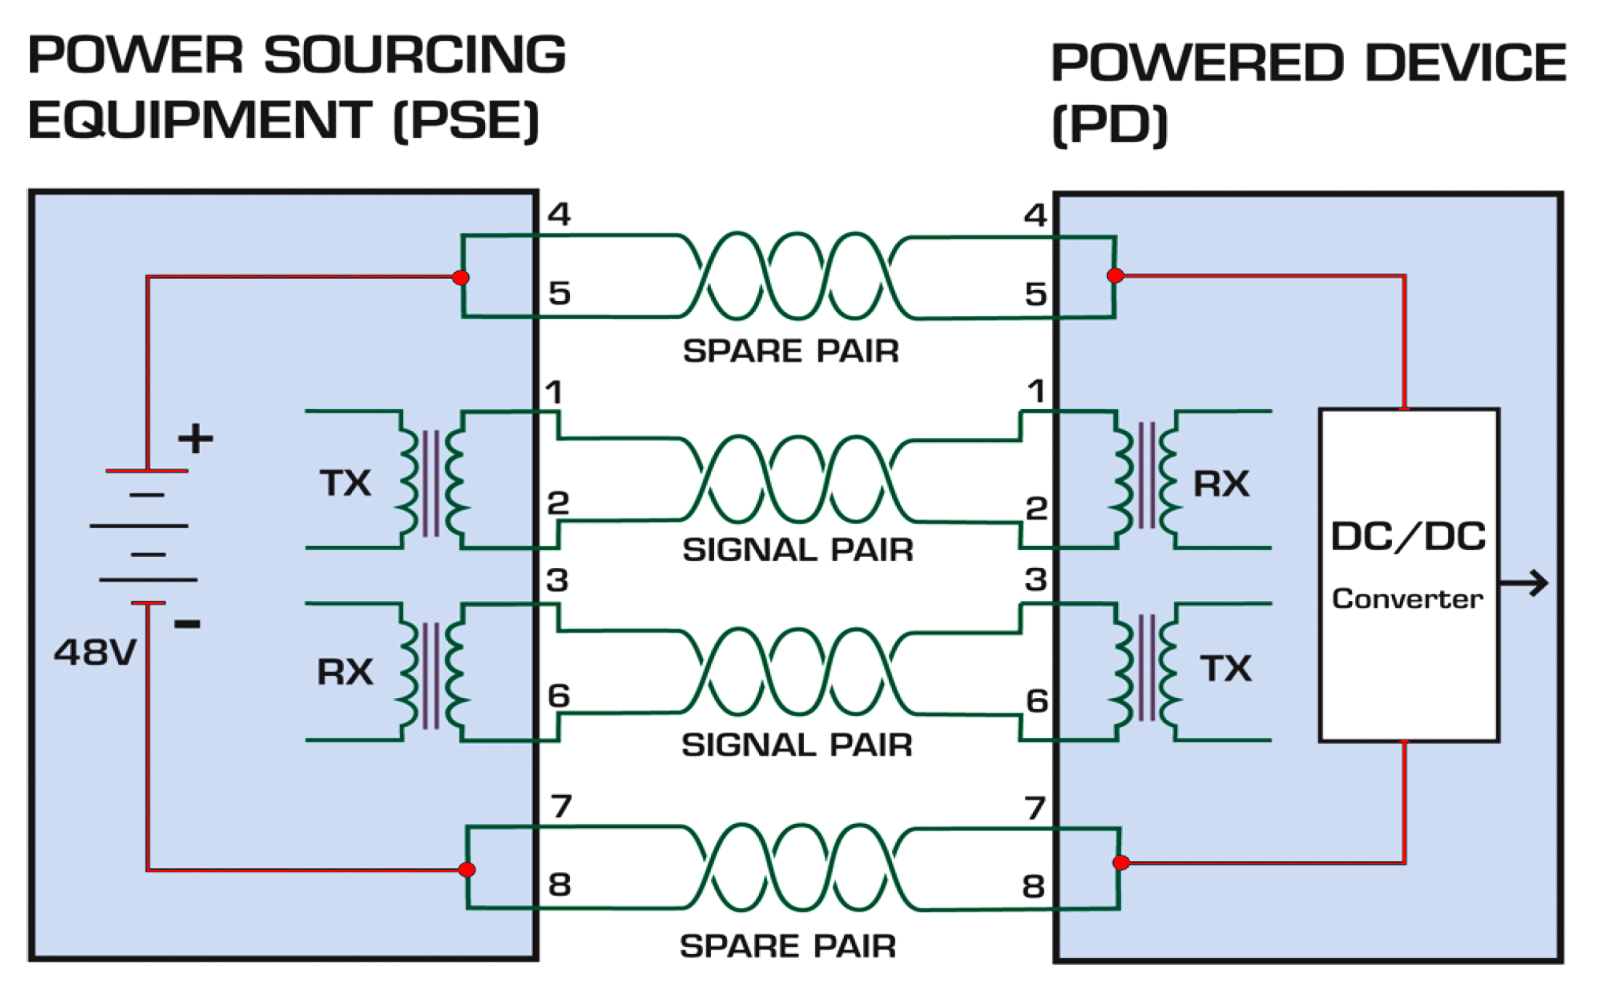
\includegraphics[width=1.0\linewidth]{figures/spare-pairs-verfahren-marked}
    \caption{Spare-Pairs-Verfahren\cite{poe1}}
    \label{fig:spare-pairs}
\end{figure}

Es gibt diesen Standard in verschiedenen Klassen. Die Default Klasse entspricht den oben beschriebenen Spezifikationen. Die anderen Klassen können teilweise auch mehr Leistung bereit stellen (bis zu ca. 21 Watt). Es gibt auch Switches, welche ca. 30 Watt pro Port bereit stellen, diese verhalten sich jedoch nicht dem Standard entsprechend.

\subsubsection{IEEE 802.3at}
Dieser Standard ist auch bei 1000Base-T Verbindungen anwendbar. Hier wird der Strom nicht in den unbenutzten Aderpaaren übertragen (die gibt es hier ja nicht), sondern der Strom wird mit dem übertragenen Daten überlagert und somit parallel übertragen. Dieses Verfahren wird \emph{Phantom-Speisung} genannt. Abbildung \ref{fig:phantom-speisung} zeigt den Aufbau dieses Verfahrens.

\begin{figure}[h]
    \centering
    \leavevmode
    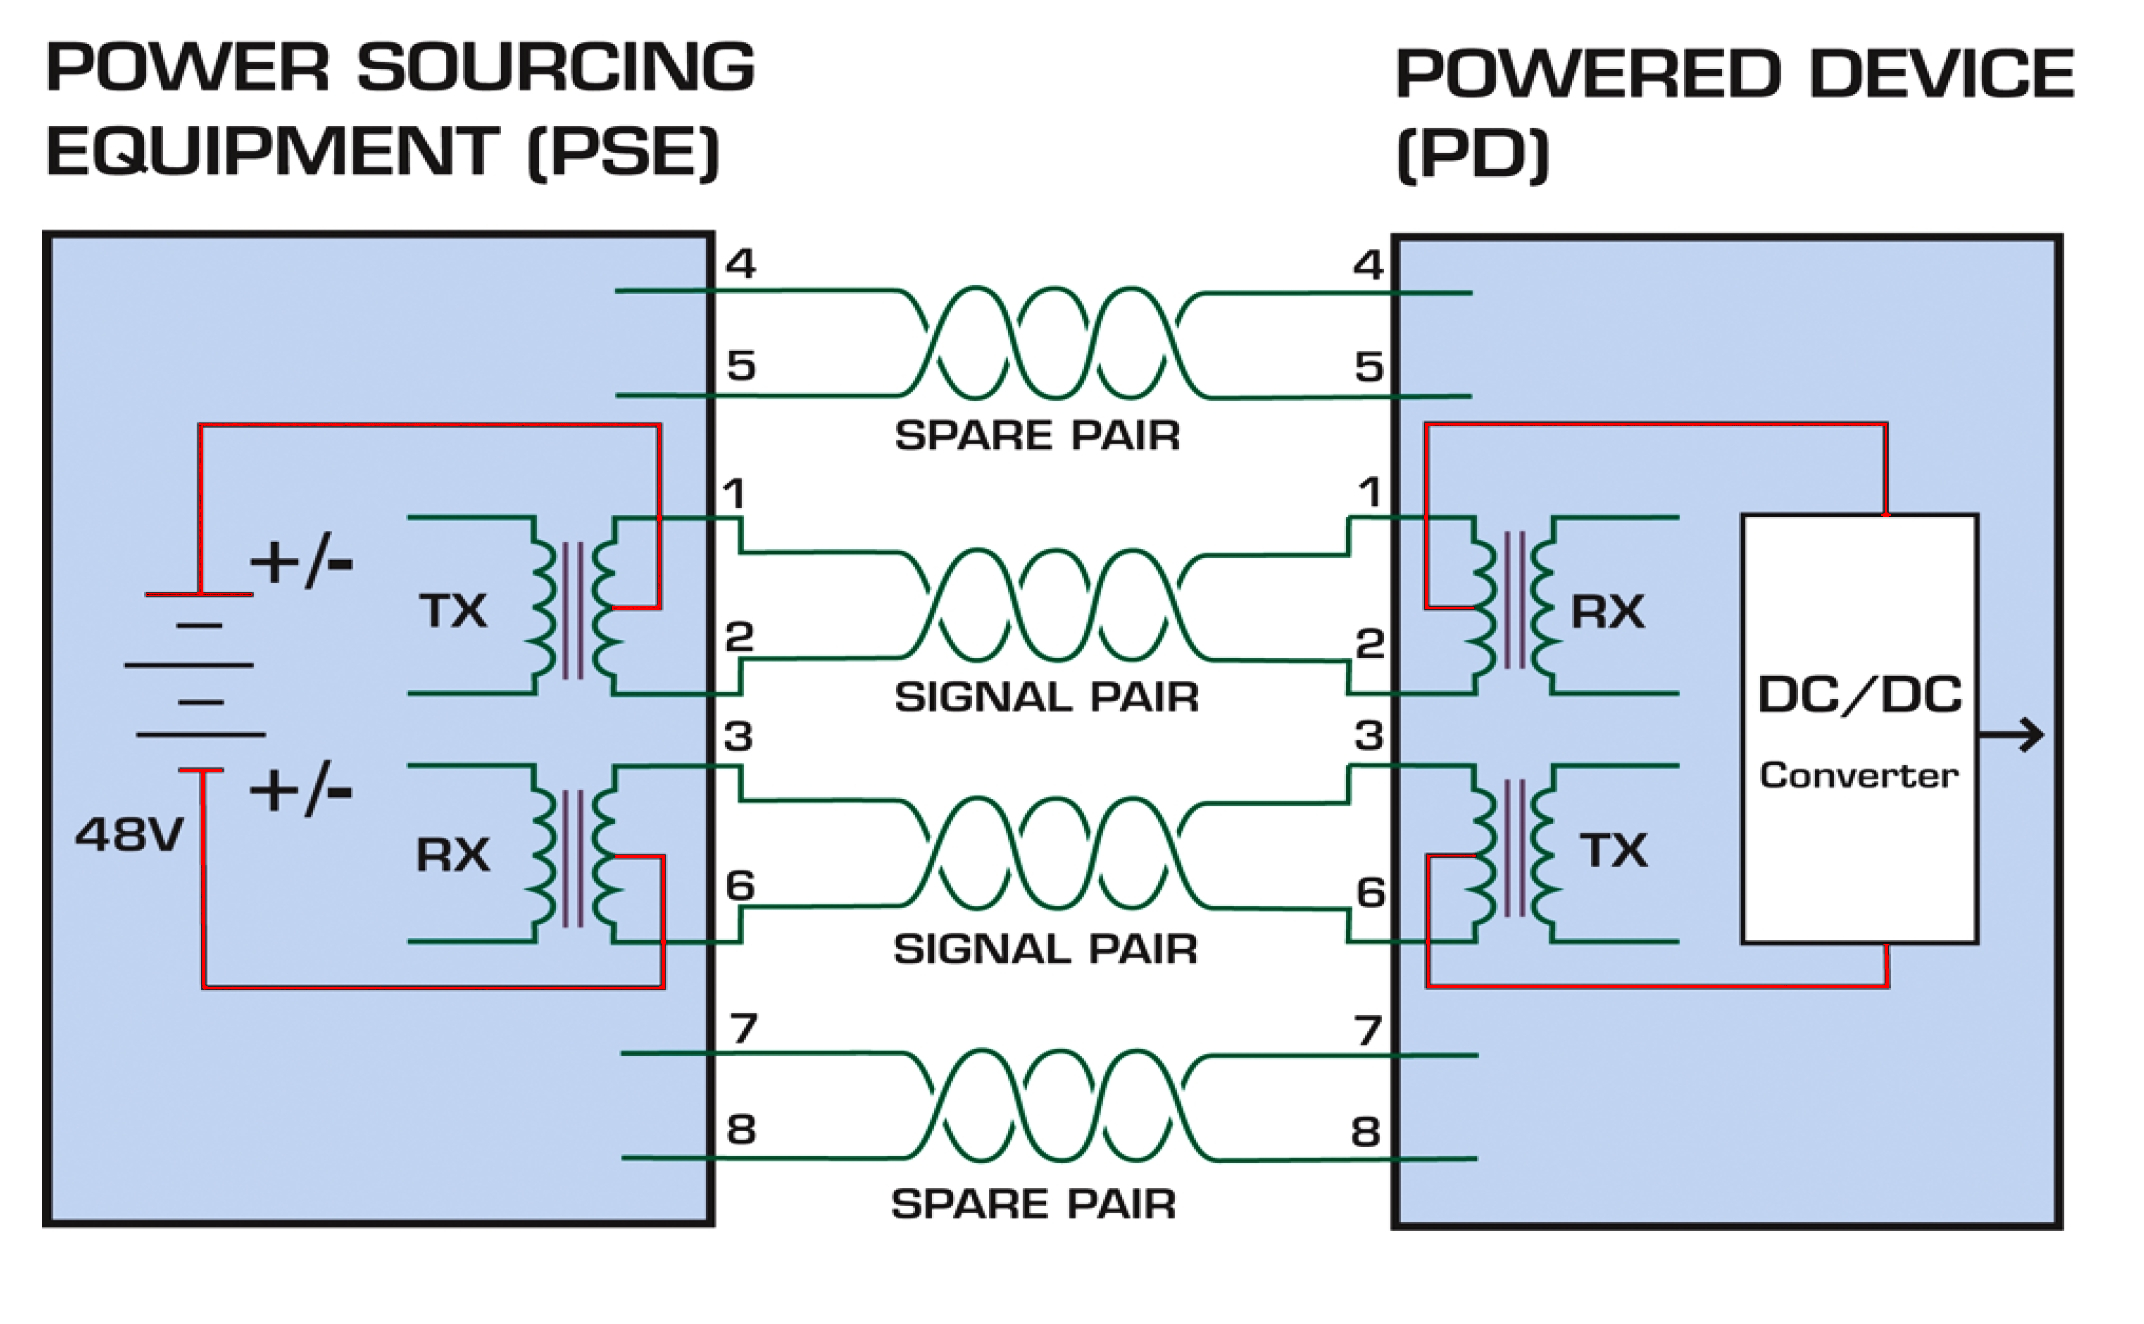
\includegraphics[width=1.0\linewidth]{figures/phantom-speisung-marked}
    \caption{Phantom-Speisung \cite{poe1}}
    \label{fig:phantom-speisung}
\end{figure}

Dieser Standard bietet höhere nutzbare Leistung, braucht aber auch bessere Kabel um richtig zu funktionieren.

\subsubsection{Energieversorgung}

Für die Versorgung der Kabel mit Strom, um sie beim Empfänger benutzen zu können, gibt es zwei Möglichkeiten\cite{poe2}:
\begin{description}
 \item[Endspan -] Es gibt direkt einen Switch welcher die Ports mit Energie versorgt.
 \item[Midspan -]Man baut auf halber Strecke (deshalb Midspan) ein zusätzliches Gerät in das Netzwerk ein, welches die Leitung mit Energie versorgt. Dies ist notwendig, solange man PoE in einen Bereich einsetzen will, in dem es noch keine PoE-fähigen Switche gibt. Das zusätzlich installierte Gerät wird auch Injector genannt.
\end{description}

Wichtiger Punkt hier ist noch, dass ein PoE Switch keine Geräte beschädigen darf, die angeschlossen sind, jedoch kein PoE unterstützen. Hierfür ist es notwendig, dass der PoE Switch erkennen kann ob ein angeschlossenes Gerät mittels PoE mit Energie versorgt werden soll oder nicht. Um dies zu gewährleisten, wurde in den IEEE Standards eine Stufe in der Kommunikationsaufbauphase hinzugefügt.

Hier wird mit kleiner Stromstärke geprüft ob der Empfänger einen gewissen Stromwiderstand hat (die Bereiche sind genau definiert). Falls ja, wird geprüft welcher PoE Standard verwendet werden soll. Danach beginnt die Speisung mit Strom und die Datenverbindung wird aufgebaut.

\subsection{SNMP}
\label{sec:SNMP}
SNMP (Simple Network Management Protocol) ist ein einfaches Mittel um Informationen Remote von einen Gerät abzufragen bzw. Remote Einstellungen an einen Gerät durchzuführen. Es wurde entworfen zu dem Zeitpunkt, an dem es mehr Computer als Experten gab und stand von Anfang an in Konkurrenz zu einen ISO standardisierten Protokoll das aber nie kam.

Simple kommt vor allem daher, dass die Entwicklung dieses Protokolls darauf abzielte eine schnell implementierte und einfache Lösung für Remote-Wartung und Monitoring zu bekommen. Es wurde sowohl bei Features (z.B. Security) als auch an dem Datentypen (es gibt eigentlich keine Datentypen, sondern es werden immer nur Bits übertragen, welche bei der anfragenden Stelle interpretiert werden müssen) gespart.

Die Kommunikation bei SNMP ist nach dem Manager/Agent Prinzip strukturiert. Agent verwaltet Ressourcen und liefert Messwerte bzw. kann Einstellungen durchführen. Manager fragt Agent nach Messwerten bzw. schickt ihm Anfragen auf Änderungen von Einstellungen.

Die Struktur der Messwerte als auch der Einstellungen die vom Agent abgefragt bzw. durch ihn geändert werden können ist intern als Baum aufgebaut. Informationen stehen nur in den Blättern (entweder skalarer Wert oder zweidimensionale Tabelle). Die Knoten sind nur für die Strukturierung der Daten wichtig.

\begin{figure}[h]
  \begin{center}
    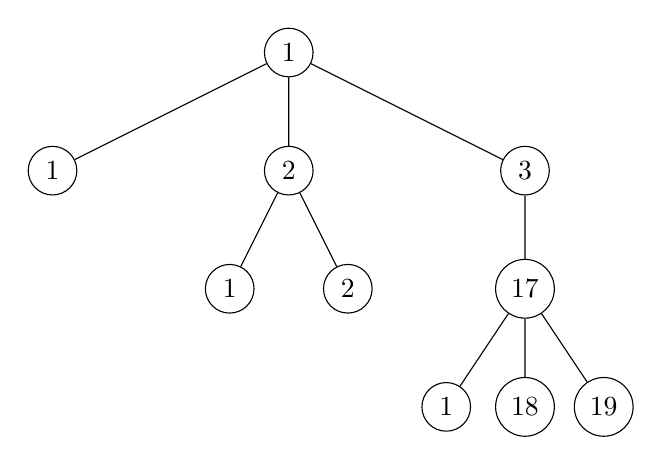
\begin{tikzpicture}[level/.style={sibling distance=30mm/#1}]
      \node [circle,draw] {$1$}
        child {node [circle,draw] {$1$}}
        child {node [circle,draw] {$2$}
          child {node [circle,draw] {$1$}}
          child {node [circle,draw] {$2$}}
        }
        child {node [circle,draw] {$3$}
          child {node [circle,draw] {$17$}
            child {node [circle,draw] {$1$}}
            child {node [circle,draw] {$18$}}
            child {node [circle,draw] {$19$}}
         }
       };
    \end{tikzpicture}
    \caption{Beispiel SNMP Baum}
    \label{fig:snmptree}
  \end{center}
\end{figure}

Abbildung \ref{fig:snmptree} zeigt ein Beispiel wie so ein Baum aussehen könnte. In diesem Baum gibt es insgesamt 6 Blätter, also können 6 Werte mit Hilfe von SNMP gelesen bzw. geändert werden. Adressiert werden die Elemente mit ihrer OID, welcher einfach den Pfad bis zum Blatt beschreibt (bsp. 1.3.17.18).

Diese Werte und deren OIDs sind zwar schön und gut, jedoch für einen Menschen praktisch unlesbar. Man müsste für jedes Gerät genau wissen unter welcher OID welche Information gespeichert ist. Dies liegt daran, dass bei der Spezifikation von SNMP keine Definition gemacht wurde, welche Information unter welcher OID gefunden werden kann.

Für diesen Grund wurde die Management Information Base (MIB) definiert. In einer solchen MIB steht, welcher OID welche Information bereit hält, welchen Typ diese Information hat usw. Hier gibt es mittlerweile schon einige definierte Gruppen. Eine Gruppe bestimmt welche OID welche Information zurück geben soll (zb. Management Gruppe, Drucker Gruppe, ...). Diese Gruppen werden normalerweise auch von den Geräten die SNMP bereitstellen unterstützt.

Die Kommunikation zwischen Manager und Agent funktioniert über Protocol Data Units (PDUs). Grundsätzlich gibt es fünf dieser PDUs in SNMP:

\begin{description}
  \item[GET\_REQUEST:] Manager stellt Agent eine Frage (z.b: Wie schnell dreht sich Lüfter A?). Als Antwort bekommt Manager ein \textbf{GET\_RESPONSE} vom Agenten.
  \item[GET\_RESPONSE:] Agent antwortet auf eine Anfrage.
  \item[SET\_REQUEST:] Manager befiehlt Agenten die Änderung an einer Einstellung (z.b: erhöhe die Drehzahl von Lüfter A). Als Antwort bekommt Manager ein \textbf{GET\_RESPONSE} vom Agenten, welche normalerweise den aktualisierten Wert enthält.
  \item[GET\_NEXT\_REQUEST:] Manager fragt den Agenten nach dem Wert der im Baum als nächstes aufgelistet ist (z.b. gib mir die Drehzahl des nächsten Lüfters). Als Antwort bekommt der Manager eine \textbf{GET\_RESPONSE} mit dem Wert vom Agenten. Da es sich aber nur um den nächsten Wert im Baum handelt, muss es nicht unbedingt sein, dass der gelesene Wert wirklich der gewünschte Wert ist (z.B. das System hat nur einen Lüfter). Um mit diesen Fällen umgehen zu können, gelten zwei Voraussetzungen:
  \begin{itemize}
    \item Manager muss wissen, dass es einen nächsten Wert gibt oder zumindest erkennen, dass der nächste Wert ihn nicht mehr interessiert (z.B. anhand der OID).
    \item Agent muss Vergleichsoperatoren beherrschen.
  \end{itemize}
  \item[TRAP:] Agent schickt zu einen vorher konfigurierten Manager eine Nachricht, falls ein bestimmter Fall eingetreten ist (z.B. der Lüfter dreht sich zu schnell → Überhitzung droht!)
\end{description}

